%<dscrpt>Graphes orientés : théorème de Mantel.</dscrpt>
Dans tout le problème \footnote{d'après \href{http://back.maquisdoc.net/v-1/index.php?act=chelt&id_elt=6651}{\emph{Modern Graph Theory}} Bela Bollobas Springer}, $\mathcal E$ désigne un ensemble fini. lorsque $\Omega$ est un ensemble fini, on notera $\sharp \, \Omega$ le nombre d'éléments de $\Omega$.

On appelle \emph{graphe orienté} une partie de $\mathcal{E}\times \mathcal{E}$ \emph{ne contenant} aucun élément de la forme $(s,s)$ pour $s\in \mathcal E$.\newline
Un graphe orienté est conventionnellement représenté par un dessin avec des cercles et des flèches. 
\begin{figure}[ht!]
 \centering
 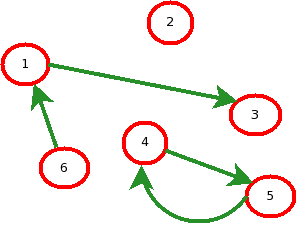
\includegraphics[width=6cm]{Emantel_1.png}
 % Emantel_1.png: 0x0 pixel, 0dpi, 0.00x0.00 cm, bb=
 \caption{Exemple de graphe orienté $\mathcal{A}$.}
 \label{fig:Emantel_1}
\end{figure}
Par exemple, le graphe orienté $\mathcal{A}$ représenté par la figure  \ref{fig:Emantel_1} est défini par :
\begin{align*}
 \mathcal{E} = \left\lbrace 1,2,3,4,5,6\right\rbrace 
& &
\mathcal A = \left\lbrace (1,3),(5,4), (6,1), (4,5)\right\rbrace 
\end{align*}
On introduit diverses définitions.
\begin{itemize}
 \item Une \emph{arête} est un élément d'un graphe orienté: c'est à dire un couple d'éléments de $\mathcal{E}$.
 \item Soit $s\in \mathcal{E}$.
\begin{itemize}
 \item On note $V_+(s)$ l'ensemble des $s'\in \mathcal{E}$ tels que $(s,s')\in\mathcal{A}$ et $d_+(s) = \sharp \, V_+(s)$ le nombre d'éléments de $V_+(s)$.
 \item On dit que $s$ est un \emph{sommet initial} lorsque $V_+(s)$ est non vide. On note $\mathcal{S}_+$ l'ensemble des sommets initiaux.
 \item On note $V_-(s)$ l'ensemble des $s'\in \mathcal{E}$ tels que $(s',s)\in\mathcal{A}$ et $d_-(s) = \sharp \, V_-(s)$ le nombre d'éléments de $V_-(s)$.
 \item On dit que $s$ est un \emph{sommet final} lorsque $V_-(s)$ est non vide. On note $\mathcal{S}_-$ l'ensemble des sommets finaux.
\end{itemize}
 \item On note $\mathcal{S}=\mathcal{S}_- \cup \mathcal{S}_+$. Un élément de $\mathcal{S}$ est appelé un \emph{sommet}.
 \item Pour toute arête $a\in\mathcal{A}$, on note $T(a) = d_-(s) + d_+(s')$ lorsque $a=(s,s')$.
\item On dira qu'un graphe orienté $\mathcal A$ est \emph{conservatif} si et seulement si
\begin{displaymath}
 \forall s \in \mathcal E : d_-(s)=d_+(s) 
\end{displaymath}
\end{itemize}

Question préliminaire.\newline
Soit $n$ un entier naturel non nul et $a_1,\cdots,a_n, b_1,\cdots,b_n$ des nombres réels quelconques. Montrer que :
\begin{displaymath}
 \left \vert \sum_{i=1}^na_i b_i \right\vert
\leq
\sqrt{\sum_{i=1}^na_i^2} \sqrt{\sum_{i=1}^nb_i^2}
\end{displaymath}


\subsection*{Partie I. Graphes orientés.}
\begin{enumerate}
\item Dans cette question seulement, le graphe orienté $\mathcal{A}$ est celui de l'exemple.
\begin{enumerate}
 \item En présentant les résultats dans un tableau, préciser $V_+(s)$, $d_+(s)$, $V_-(s)$, $d_-(s)$ pour chaque $s\in \mathcal{E}$.
 \item Préciser les ensembles $\mathcal{S}_-$, $\mathcal{S}_+$, $\mathcal{S}$.
 \item Le graphe est-il conservatif ?
\end{enumerate}  

\item Soit $\mathcal{A}$ un graphe orienté.
\begin{enumerate}
 \item Préciser les ensembles
\begin{align*}
 \bigcup_{s\in\mathcal{S}_+}\left\lbrace (s,s'), s'\in V_+(s)\right\rbrace
& &
 \bigcup_{s\in\mathcal{S}_-}\left\lbrace (s',s), s'\in V_-(s)\right\rbrace 
\end{align*}
\item Montrer que 
\begin{displaymath}
 \sharp \, \mathcal{A} =
\sum_{s\in \mathcal S_+}d_+(s) = \sum_{s\in \mathcal S_-}d_-(s)
\end{displaymath}

\end{enumerate}


\item Soit $\mathcal{A}$ un graphe orienté. Montrer que
\begin{align*}
 \sum_{(s,s')\in \mathcal A}d_+(s') = \sum _{s'\in \mathcal S_-}d_-(s')d_+(s')
&  &
 \sum_{(s,s')\in \mathcal A}d_-(s) = \sum _{s\in \mathcal S_+}d_-(s)d_+(s)
\end{align*}

\item On dit qu'un graphe orienté $\mathcal{A}$ \emph{contient un triangle} si et seulement si
\begin{displaymath}
 \exists (s_1,s_2,s_3)\in \mathcal{S}^3 \text{ tel que :}
\left\lbrace
\begin{aligned}
 (s_1,s_2) &\in \mathcal{A} \\
 (s_2,s_3) &\in \mathcal{A} \\
 (s_3,s_1) &\in \mathcal{A} 
\end{aligned}
 \right. 
\end{displaymath}
\begin{enumerate}
 \item Montrer que $\mathcal A$ contient un triangle si et seulement si
\begin{displaymath}
 \exists (s,s')\in \mathcal{A} \text{ tel que } V_+(s')\cap V_-(s) \neq \emptyset
\end{displaymath}

\item Montrer que si $\mathcal{A}$ ne contient pas de triangle alors $T(a) \leq \sharp \, \mathcal S$ pour toute arête $a$.
\end{enumerate}

\item Montrer que, si $\mathcal A$ est un graphe orienté conservatif,
\begin{displaymath}
 \sqrt{2}\; \sharp \, \mathcal{A} \leq \sqrt{\sharp \, \mathcal{S} \,\sum_{a\in \mathcal A}T(a)}
\end{displaymath}

\item Théorème de Mantel (1907).\newline
Soit $\mathcal A$ un graphe orienté conservatif. Montrer que si
\begin{displaymath}
 \sharp \, \mathcal A > \frac{1}{2} (\,\sharp \, \mathcal S )^2
\end{displaymath}
alors $\mathcal A$ contient un triangle.
\end{enumerate}

\subsection*{Partie II. Graphes non orientés.}
On définit un \emph{graphe non orienté} comme étant un ensemble de \emph{paires} (parties à deux éléments) d'un ensemble $\mathcal E$.
\begin{enumerate}
\item Comment peut-on définir simplement un graphe orienté $\mathcal A$ à partir d'un graphe non orienté $\mathcal O$ ? Que peut-on dire des ensembles de sommets ? Quelle propriété $\mathcal A$ possède-t-il automatiquement ? Former une relation entre les nombres d'arêtes.
\item Formulez et démontrez un résultat analogue au théorème de Mantel pour un graphe non orienté.

\begin{figure}[ht!]
 \centering
 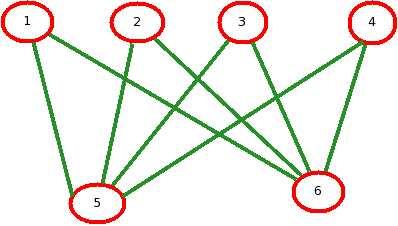
\includegraphics[width=6cm]{Emantel_2.png}
 % Emantel_1.png: 0x0 pixel, 0dpi, 0.00x0.00 cm, bb=
 \caption{Graphe bipartite complet.}
 \label{fig:Emantel_2}
\end{figure}

\item Lorsque l'ensemble $\mathcal{E}$ est une union disjointe de deux ensembles $\mathcal E_1$ (contenant $n_1$ éléments) et $\mathcal E_2$ (contenant $n_2$ éléments), on définit un graphe non orienté $\mathcal B$ (appelé \emph{graphe bipartite complet}) par :
\begin{itemize}
 \item chaque élément de $\mathcal E_1$ est relié à chaque élément de $\mathcal E_2$.
 \item il n'existe aucune liaison entre deux éléments de $\mathcal E_1$.
 \item il n'existe aucune liaison entre deux éléments de $\mathcal E_2$.
\end{itemize}
Calculer $\sharp\, \mathcal B$.
\item Soit $n$ un entier naturel non nul quelconque.\newline
Montrer qu'il existe un graphe non orienté tel que :
\begin{itemize}
 \item le nombre de sommets est $n$
 \item il ne contient pas de triangle
 \item le nombre d'arêtes est la partie entière de $\frac{n^2}{4}$.
\end{itemize} 
On pourra séparer les cas pairs et impairs pour le nombre de sommets.
\end{enumerate}


